\begin{hcarentry}{Haskino}
\label{Haskino}
\report{Mark Grebe}%10/15
\participants{Andy Gill}
\status{active}
\makeheader

%**<img width=400 src="./jh2.jpg">
%*ignore
\begin{center}
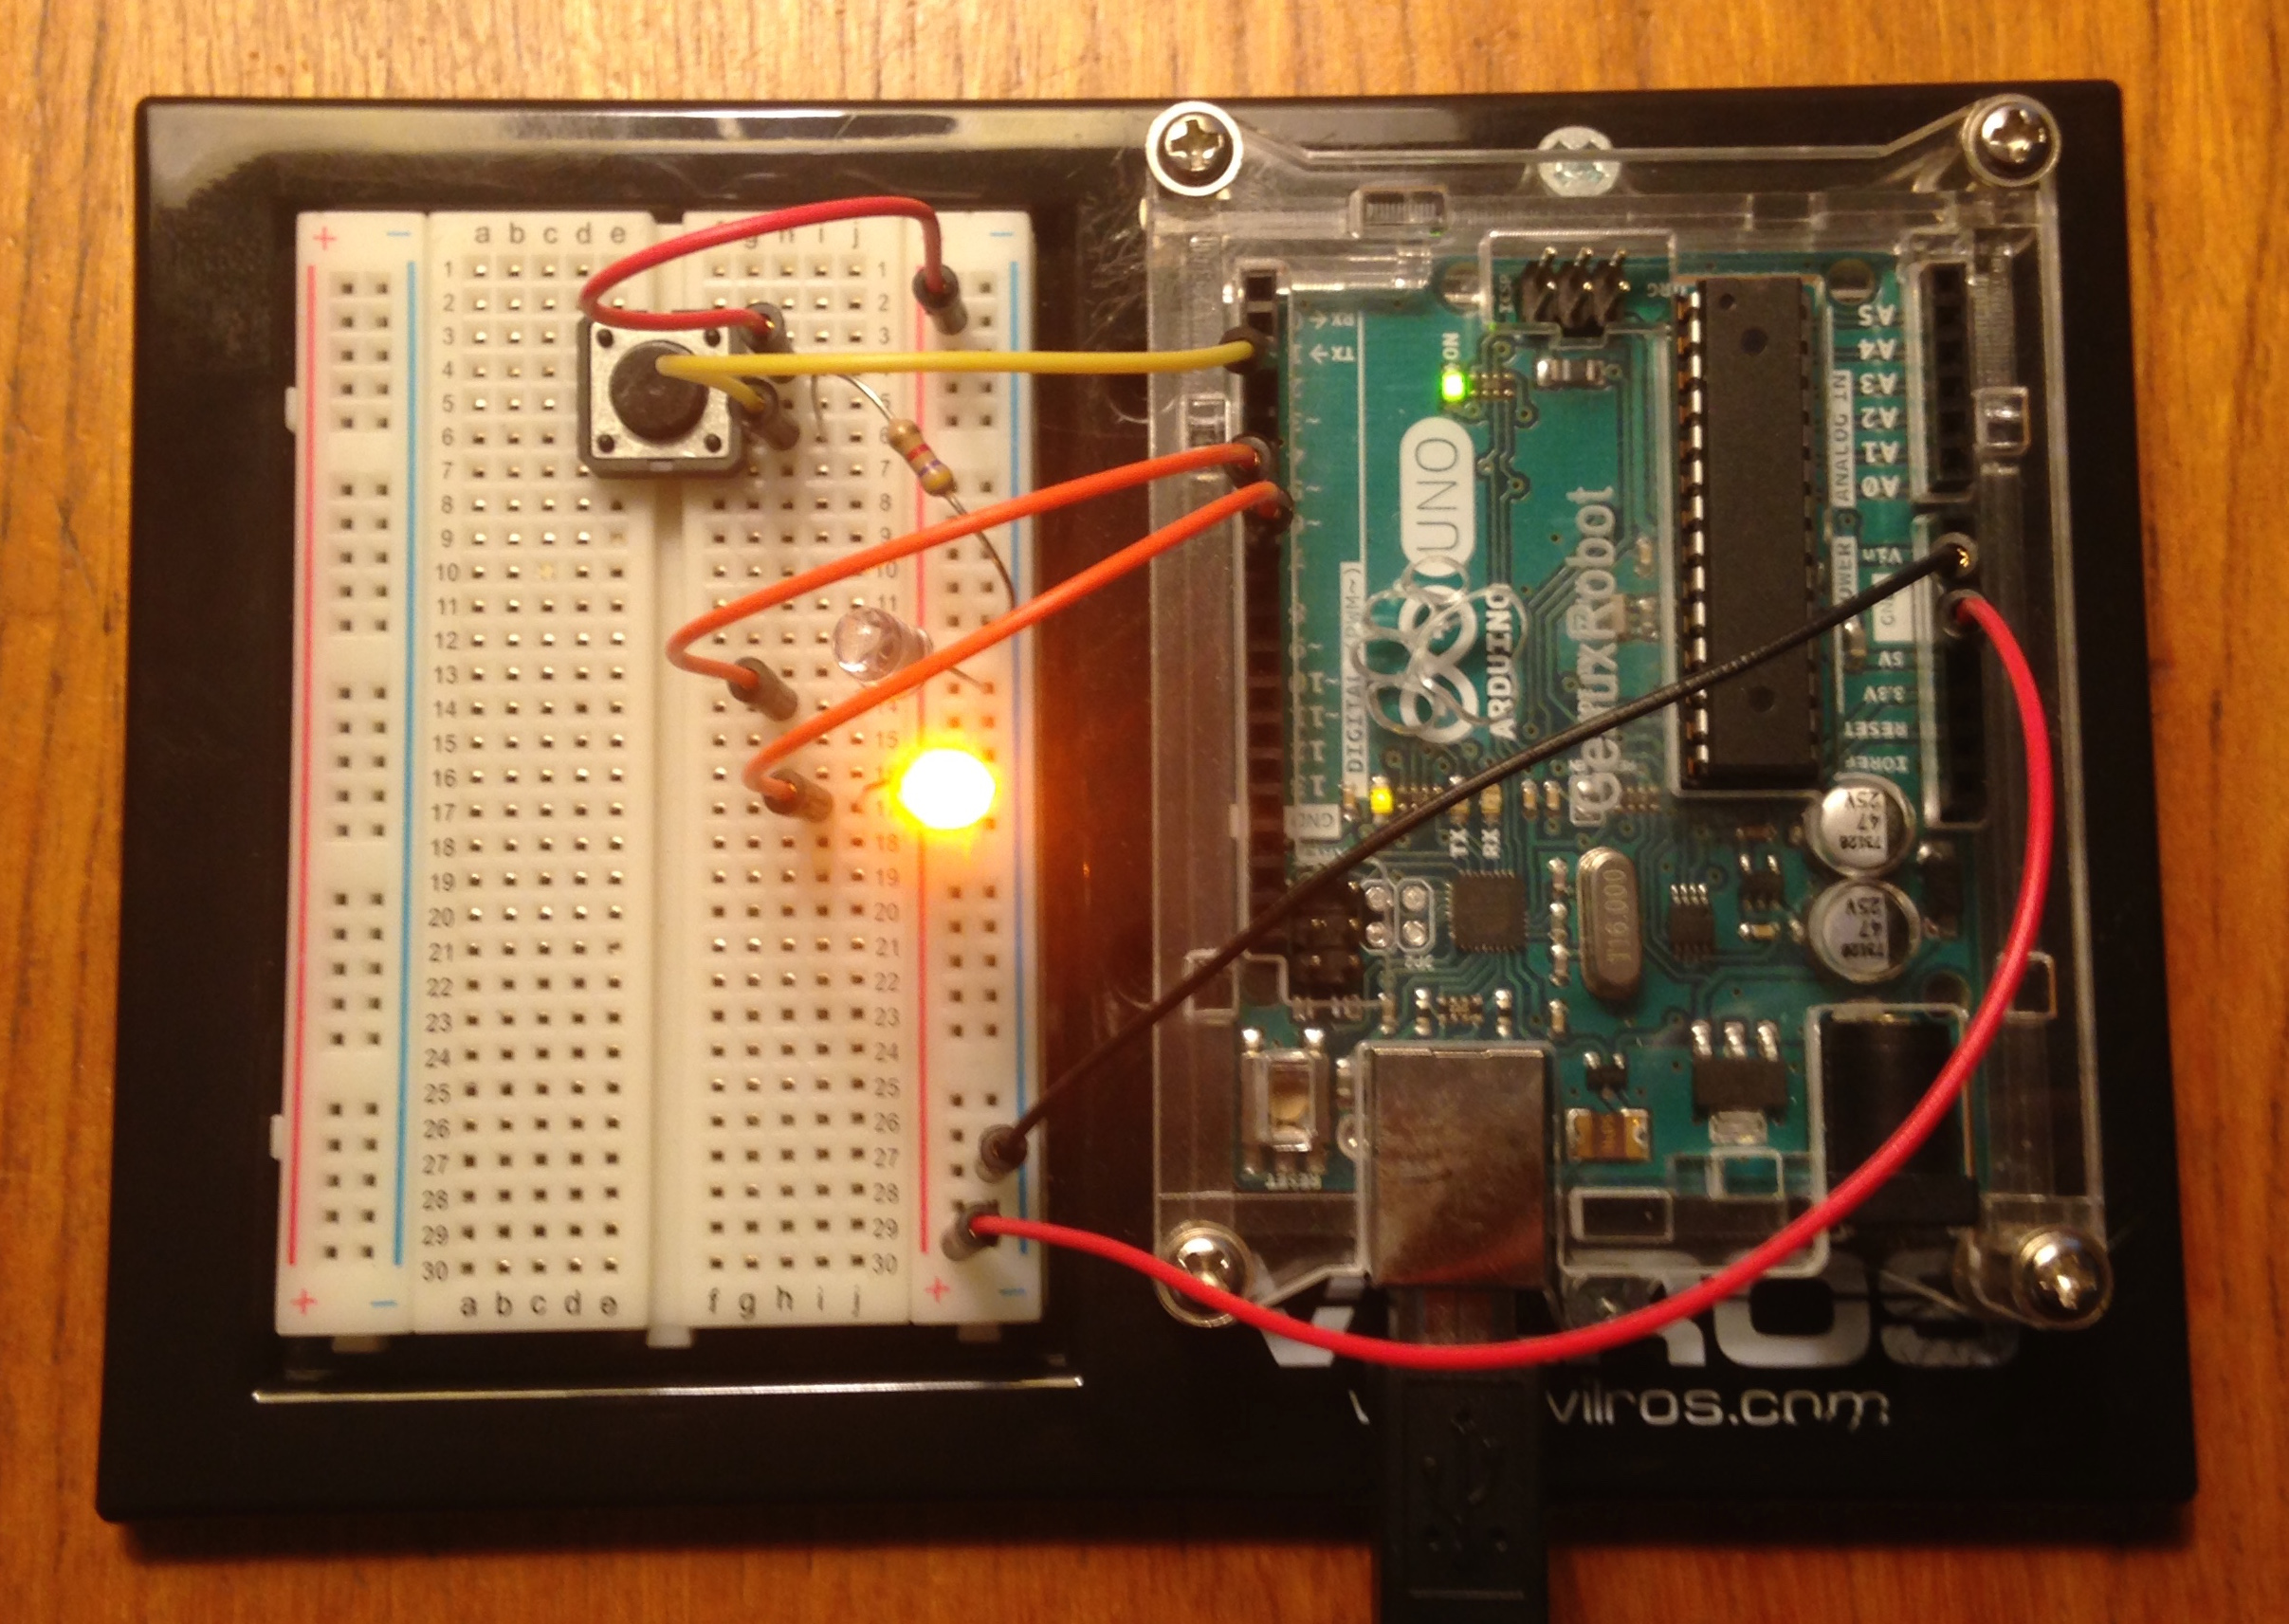
\includegraphics[width=0.435\textwidth]{html/Arduino.jpg}
\end{center}
%*endignore


Haskino is a Haskell development environment for programming the
Arduino microcontroller boards in a high level functional language
instead of the low level C language normally used.  Haskino presents
two complimentary ways of developing programs for the Arduino.

The first method allows programming of an Arduino tethered to a host
computer through a serial connection.  This work started with Levent
Erk\"{o}k's hArduino package.  To this we have added our strong Remote
Monad concepts, which provide a more efficient method of communication
with the board.  We have also replaced the Firmata serial
communication protocol and firmware with a new protocol and firmware
which also allow for more efficient communication, and are expandable
to meet the needs of our second programming method.

The second method of programming the Arduino uses a deep embedding to
out-source entire groups of commands and control-flow idioms.  These
programs may then be stored in EEPROM on the board, and executed from
startup, with no connection to the host computer required.  A Haskell
programmer can start program development with the first method, which
allows for convenient prototyping and debugging.  The program can then
be moved to the second method, with the entire computation being
performed on the Arduino, and not requiring the host computer.

The development has been active over the past 6 months and there is a
paper accepted for publication in PADL 2016.

\FurtherReading
\begin{compactitem}
\item
  \url{https://github.com/ku-fpg/haskino}
\item
  \url{https://github.com/ku-fpg/wiki}
\end{compactitem}
\end{hcarentry}
